\documentclass[tikz,png]{standalone}
\usepackage{unicode-math}
\usetikzlibrary{positioning}
\begin{document}
  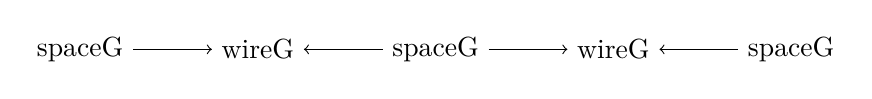
\begin{tikzpicture}
    \node (spaceG) {spaceG};
    \node[right = of spaceG] (wireG) {wireG};
    \node[right = of wireG] (spaceG') {spaceG};
    \node[right = of spaceG'] (wireG') {wireG};
    \node[right = of wireG'] (spaceG'') {spaceG};

    \draw[->] (spaceG) -- (wireG);
    \draw[->] (spaceG') -- (wireG);
    \draw[->] (spaceG') -- (wireG');
    \draw[->] (spaceG'') -- (wireG');
  \end{tikzpicture}
\end{document}
